\usetikzlibrary{math}
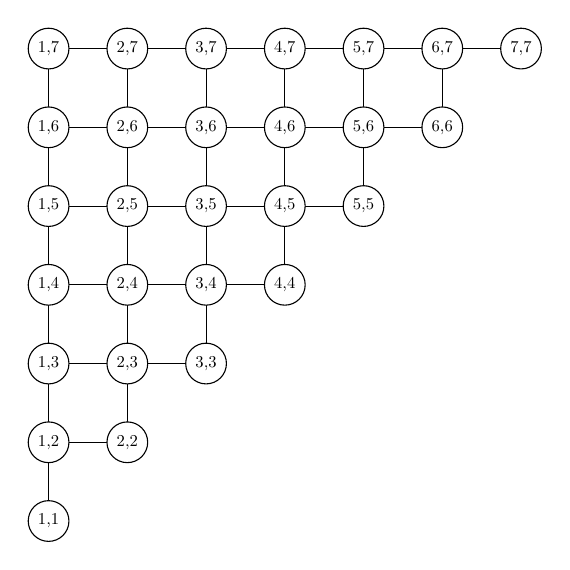
\begin{tikzpicture}
\tikzstyle{dot}=[draw,circle,fill=white,scale=0.6];
\foreach \x in {2,...,7}{
	\foreach \y in {\x,...,7}{
		\draw (\x-1,\y-1)--(\x-1,\y);
		\draw (\x,\y)--(\x-1,\y);
	}
}

\foreach \x in {1,...,7}{
	\foreach \y in {\x,...,7}{
		\node[dot] at (\x,\y) {\x,\y};
	}
}
\end{tikzpicture}